% This is samplepaper.tex, a sample chapter demonstrating the
% LLNCS macro package for Springer Computer Science proceedings;
% Version 2.20 of 2017/10/04
%
\documentclass[runningheads]{llncs}
%
\usepackage{graphicx}
\usepackage{todonotes}
\usepackage{hyperref}
\usepackage{tabularx}
\usepackage{array}
% Used for displaying a sample figure. If possible, figure files should
% be included in EPS format.
%
% If you use the hyperref package, please uncomment the following line
% to display URLs in blue roman font according to Springer's eBook style:
% \renewcommand\UrlFont{\color{blue}\rmfamily}

\begin{document}
%
\title{Assignment 2: A Real Life Competition}
%
%\titlerunning{Abbreviated paper title}
% If the paper title is too long for the running head, you can set
% an abbreviated paper title here
%
\author{Group 162: Vesper Kukler 2747734 \and
Antonio Pascarella 2895210 \and
Alessandro Bertoncini 2903205}
%
\authorrunning{V. Kukler et al.}
% First names are abbreviated in the running head.
% If there are more than two authors, 'et al.' is used.
%
\institute{Vrije Universiteit Amsterdam, Amsterdam, The Netherlands}
%
\maketitle              % typeset the header of the contribution
%
%
%
%
\section{First Section}
\subsection{A Subsection Sample}
Please note that the first paragraph of a section or subsection is
not indented. The first paragraph that follows a table, figure,
equation etc. does not need an indent, either.

Subsequent paragraphs, however, are indented.

\subsubsection{Sample Heading (Third Level)} Only two levels of
headings should be numbered. Lower level headings remain unnumbered;
they are formatted as run-in headings.

\paragraph{Sample Heading (Fourth Level)}
The contribution should contain no more than four levels of
headings. Table~\ref{tab1} gives a summary of all heading levels.

\begin{table}
\caption{Table captions should be placed above the
tables.}\label{tab1}
\begin{tabular}{|l|l|l|}
\hline
Heading level &  Example & Font size and style\\
\hline
Title (centered) &  {\Large\bfseries Lecture Notes} & 14 point, bold\\
1st-level heading &  {\large\bfseries 1 Introduction} & 12 point, bold\\
2nd-level heading & {\bfseries 2.1 Printing Area} & 10 point, bold\\
3rd-level heading & {\bfseries Run-in Heading in Bold.} Text follows & 10 point, bold\\
4th-level heading & {\itshape Lowest Level Heading.} Text follows & 10 point, italic\\
\hline
\end{tabular}
\end{table}


\noindent Displayed equations are centered and set on a separate
line.
\begin{equation}
x + y = z
\end{equation}
Please try to avoid rasterized images for line-art diagrams and
schemas. Whenever possible, use vector graphics instead (see
Fig.~\ref{fig1}).

\begin{figure}
\includegraphics[width=\textwidth]{fig1.eps}
\caption{A figure caption is always placed below the illustration.
Please note that short captions are centered, while long ones are
justified by the macro package automatically.} \label{fig1}
\end{figure}

\begin{theorem}
This is a sample theorem. The run-in heading is set in bold, while
the following text appears in italics. Definitions, lemmas,
propositions, and corollaries are styled the same way.
\end{theorem}
%
% the environments 'definition', 'lemma', 'proposition', 'corollary',
% 'remark', and 'example' are defined in the LLNCS documentclass as well.
%
\begin{proof}
Proofs, examples, and remarks have the initial word in italics,
while the following text appears in normal font.
\end{proof}
For citations of references, we prefer the use of square brackets
and consecutive numbers. Citations using labels or the author/year
convention are also acceptable. The following bibliography provides
a sample reference list with entries for journal
articles~\cite{ref_article1}, an LNCS chapter~\cite{ref_lncs1}, a
book~\cite{ref_book1}, proceedings without editors~\cite{ref_proc1},
and a homepage~\cite{ref_url1}. Multiple citations are grouped
\cite{ref_article1,ref_lncs1,ref_book1},
\cite{ref_article1,ref_book1,ref_proc1,ref_url1}.

\section{Business Understanding}

\color{blue}Your task is to predict what hotel properties that result from a search of a user, the user is
most likely to click on. Of course, more people have worked on such predictions. Can you
find some other people that have tried to make such predictions (e.g. from the Kaggle com-
petition)? And what have they used as most prominent predictors? Have other people that
participate in the competition mentioned anything about their approaches? Please spend a
couple of paragraphs on this topic in a ’Related Work’ section in your report.\color{black}

\subsection{Business Context}

We are focusing on a recommender system, a specific AI-based tool that suggests products, items, or content to users. In this case, it is a hotel-filtering tool that presents different accommodation options based on the user’s requests.

Today, most travelers rely on platforms like Expedia or Booking to select the best hotel in terms of quality and price. For this reason, it is crucial for hospitality businesses to appear on these websites. In addition, ranking is a key factor: users are unlikely to scroll through all the listings, so the options shown at the top are far more likely to be chosen.

\subsection{Business Problem}

The core challenge is to identify the factors that influence users’ choices. In particular, this understanding enables booking platforms to present options that closely match users’ preferences and requirements. As a result, Expedia (or Booking, etc.) can achieve higher conversion rates, hotels can increase their revenue, and customers are more satisfied. In other words, it is a win-win scenario: the user quickly finds exactly what they are looking for with the minimum number of clicks.

\subsection{Data Mining Objectives}

At this stage, we will focus on the following objectives:
\begin{itemize}
    \item \textit{Understand, Analyze and Elaborate Data}: We must first clarify the overall context: what data do we have? Does it accurately describe the situation? Does it require further enrichment, and if so, in what way?
    \item \textit{Feature Selection}: Determine the most relevant attributes that can be used as features for training and evaluating the model.
    \item \textit{Build the Model (and iterate if necessary)}: Because we need to generate a detailed ranking list in response to users’ queries, we will develop a classification model capable of assigning one of the following labels to hotel properties: \textbf{booked}, \textbf{clicked}, \textbf{ignored}. The results will then be benchmarked against Normalized Discounted Cumulative Gain (NDCG)@5 calculated per query and averaged over all queries with the values weighted by the $log_2$
function.
\end{itemize}

\subsection{Success Criteria and Constraints}

"\texttt{The winner will be rewarded with the fame and glory of winning the 2026VU Data Mining Techniques cup.}" This sounds quite enticing, doesn't it? To this end, we strive to obtain the highest possible score according to the NDCG evaluation metric. At the same time, we also aim to secure strong precision and recall values.

\subsection{Related Work}

One of the most compelling solutions proposed for this specific problem uses a collection of machine learning models whose predictions are then aggregated through several ensemble methods \cite{DBLP:journals/corr/LiuXZYPLSW13}. The following key ideas from that work could be integrated into our approach:
\begin{itemize}
    \item \textbf{Validation Set and Class Balance: }around 10\% of the training data is set aside as a validation set to compare and tune the models. In addition, because tree-based methods and neural networks are sensitive to class imbalance, the training data is constructed to have a 1:1 ratio of positive to negative examples. Here, a positive example indicates that the hotel was booked or clicked, while a negative example indicates that it was ignored.
    \item \textbf{Composite Features: }this is a standard step in feature engineering. Certain features become more informative when combined. In this case, a new feature called \textit{count\_window} is defined to jointly represent both “number of rooms” and “booking lead time” in a single value, potentially enabling some models to better learn the interaction between these two aspects.
    \item \textbf{Per-Country Splitting: }to accelerate the training of tree-based models, the dataset is partitioned by country, yielding 172 separate subsets. An independent model is then trained on each subset. This not only reduces training time but also aligns with the intuition that hotels within the same country are likely to exhibit similar behavior.
    \item \textbf{Handling Missing Values: }within each country-specific subset, the first quartile of a feature’s distribution is computed and used to impute missing values. Compared to mean imputation, this approach is more robust in the presence of outliers.
\end{itemize}


\section{Data Understanding}

\color{blue}In this task, you will do some exploratory data analysis (EDA). Explore the dataset, count, summarize, plot things, and report findings that are useful for creating predictions. Remember that EDA is not necessarily done once at the start of the project. It is expected that you do some EDA, build some features, train some models, then some idea comes up, do some more EDA, modify your features, train another model on these new features, and so on.\color{black}

\subsection{Dataset Overview}
The training dataset contains a total of 4,958,347 rows, corresponding to 199,795 distinct searches conducted over approximately 241 days (from 1 November 2012 to 30 June 2013). Reporting the number of rows with missing values is not very informative, as every record has at least one missing field. It is also worth noting that the training set includes some attributes that are not present in the test set:

\begin{table}[ht]
\centering
\renewcommand{\arraystretch}{1.15}

\begin{tabularx}{\textwidth}{@{}%
    >{\raggedright\arraybackslash}p{0.24\textwidth}
    >{\raggedright\arraybackslash}p{0.14\textwidth}
    X@{}}
\hline
& \multicolumn{2}{c}{\textbf{Training set only}} \\
\hline
position & Integer &
Hotel position on Expedia's search results page. This is only provided for the training data, but not the test data \\
\hline
click\_bool & Boolean &
1 if the user clicked on the property, 0 if not \\
\hline
booking\_bool & Boolean &
1 if the user booked the property, 0 if not \\
\hline
gross\_booking\_usd & Float &
Total value of the transaction. This can differ from the price\_usd due to taxes, fees, conventions on multiple day bookings and purchase of a room type other than the one shown in the search \\
\hline
\end{tabularx}

\end{table}

Furthermore, there are 129,113 unique hotels, of which 51,768 belong to a major chain while the remaining 77,345 are independent ones. They are spread across 172 countries, whereas customers engaged with Expedia from 210 different countries.

\subsection{Target Distribution and Query Structure}
Each query returns between 5 and 38 results, with a median of 29. The two target labels are highly imbalanced: only 4.47\% of rows are clicked and 2.79\% are booked. Per query, most users click on a single property (186,764 out of 199,795 queries with at least one click) and book at most one (138,390 queries contain a booking, the remaining 61,405 do not). This imbalance motivates the 1:1 down-sampling strategy proposed by \cite{DBLP:journals/corr/LiuXZYPLSW13} and is consistent with the use of NDCG@5 as evaluation metric, since most of the relevance mass is concentrated on the top results.

\begin{figure}[ht]
\centering
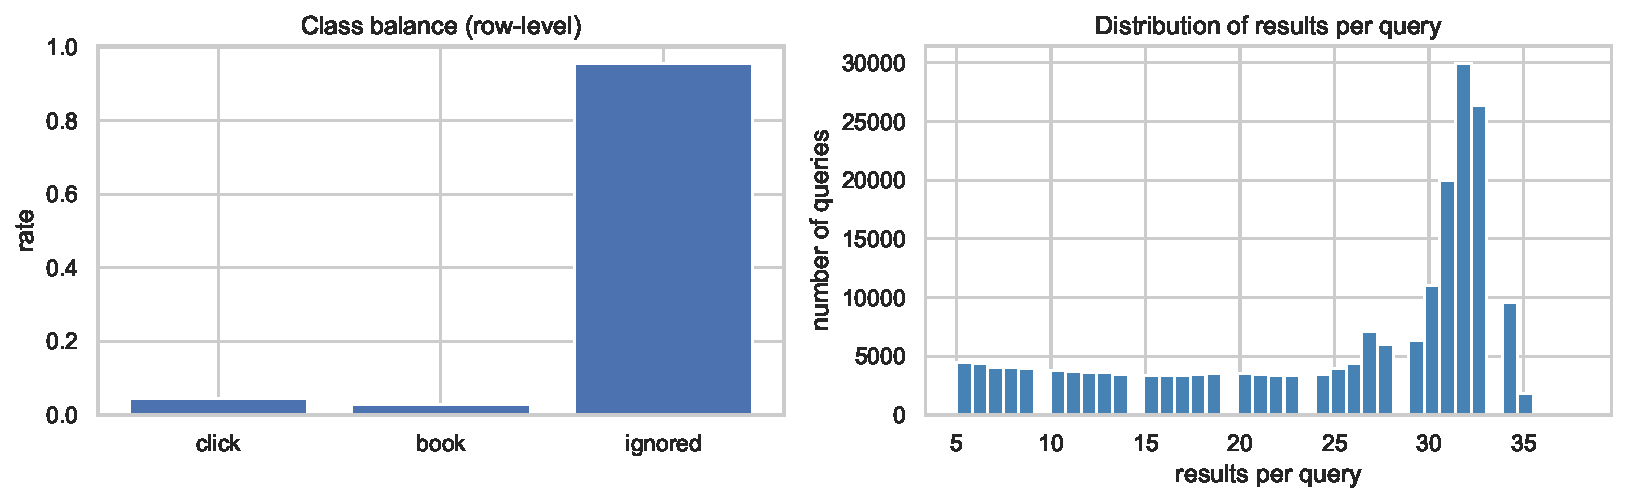
\includegraphics[width=\textwidth]{figures/target_distribution.pdf}
\caption{Class balance at row level (left) and distribution of the number of results per query (right).}
\label{fig:target}
\end{figure}

\subsection{Position Bias}
About 29.6\% of queries are returned in random order (\texttt{random\_bool}=1), while the remaining ones use Expedia's default sort. Comparing click-through and booking rates across positions for the two groups isolates the position bias from the true relevance signal (Fig.~\ref{fig:position}). For Expedia-sorted queries the engagement decays sharply with position; for random queries the decay is much milder. We will exploit this difference when training the ranker, either by relying on the random-sorted subset for evaluation or by applying a position-aware weighting.

\begin{figure}[ht]
\centering
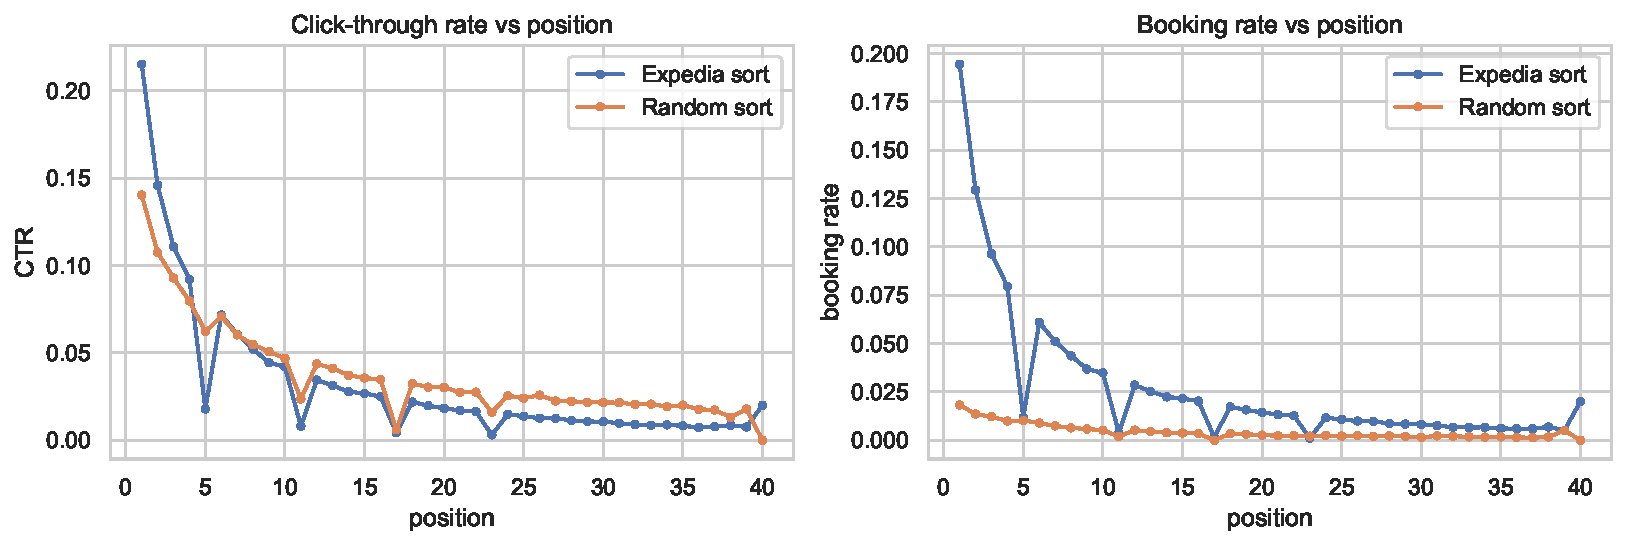
\includegraphics[width=\textwidth]{figures/position_bias.pdf}
\caption{Click-through rate (left) and booking rate (right) by position, split by sort type.}
\label{fig:position}
\end{figure}

\subsection{Price Patterns}
The \texttt{price\_usd} column has a long right tail: the median is \$122, the 99th percentile is \$599, but the maximum reaches \$1.97\,M and 2,871 rows exceed \$5,000. There are also 31 rows with a price of zero. These extremes are likely encoding errors and will be clipped or removed during preparation. More importantly, the \emph{relative} price within a query is a much stronger signal than the absolute one: ranking the cheapest option first within each search yields a clear monotonic decay of CTR and booking rate with the price rank (Fig.~\ref{fig:price}). We therefore plan to engineer a \texttt{price\_rank\_in\_query} feature.

\begin{figure}[ht]
\centering
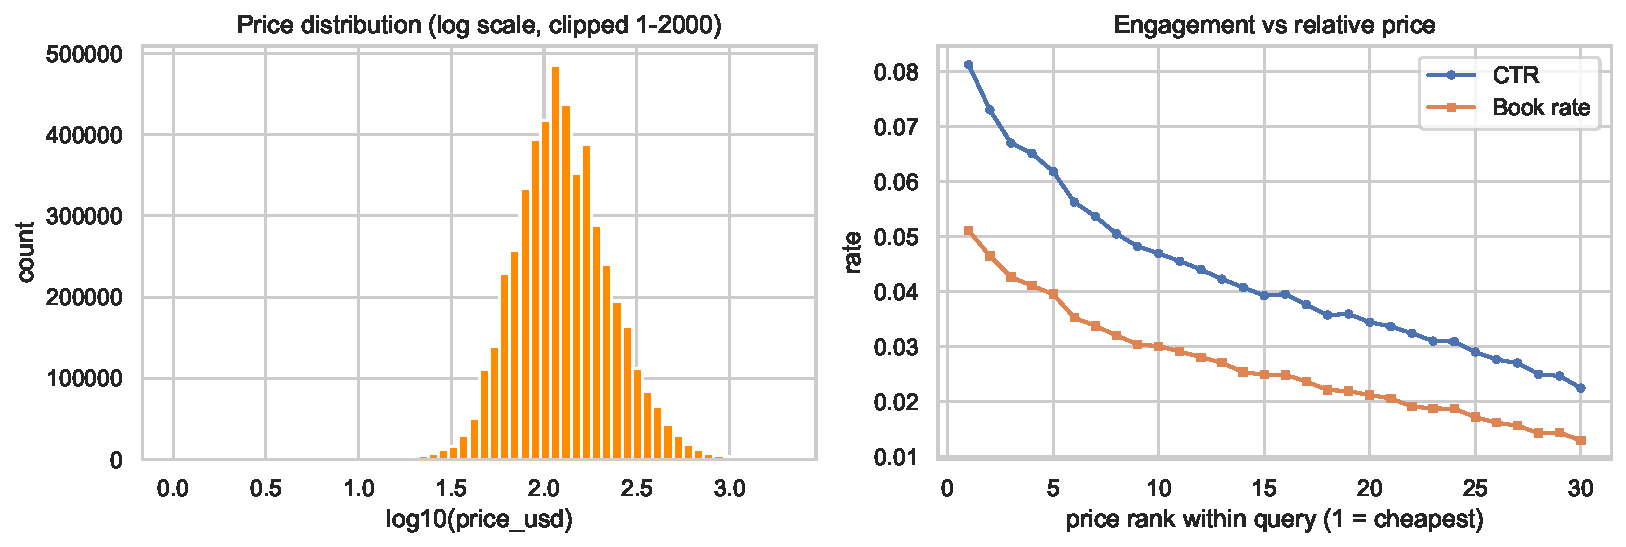
\includegraphics[width=\textwidth]{figures/price_patterns.pdf}
\caption{Price distribution on a log scale (left) and engagement by price rank within the query (right).}
\label{fig:price}
\end{figure}

\subsection{Property Quality}
Engagement increases with both star rating and review score, peaking at four-star properties (CTR 5.4\%, booking rate 3.3\%), and dips slightly for five-star ones, probably because of the higher price. The \texttt{prop\_brand\_bool} flag has only a small effect (chain hotels are booked slightly more often: 2.92\% vs 2.57\%), while the \texttt{promotion\_flag} produces a large lift (CTR 6.0\% vs 4.0\%, booking rate 3.9\% vs 2.5\%). These features are clearly useful for ranking.

\begin{figure}[ht]
\centering
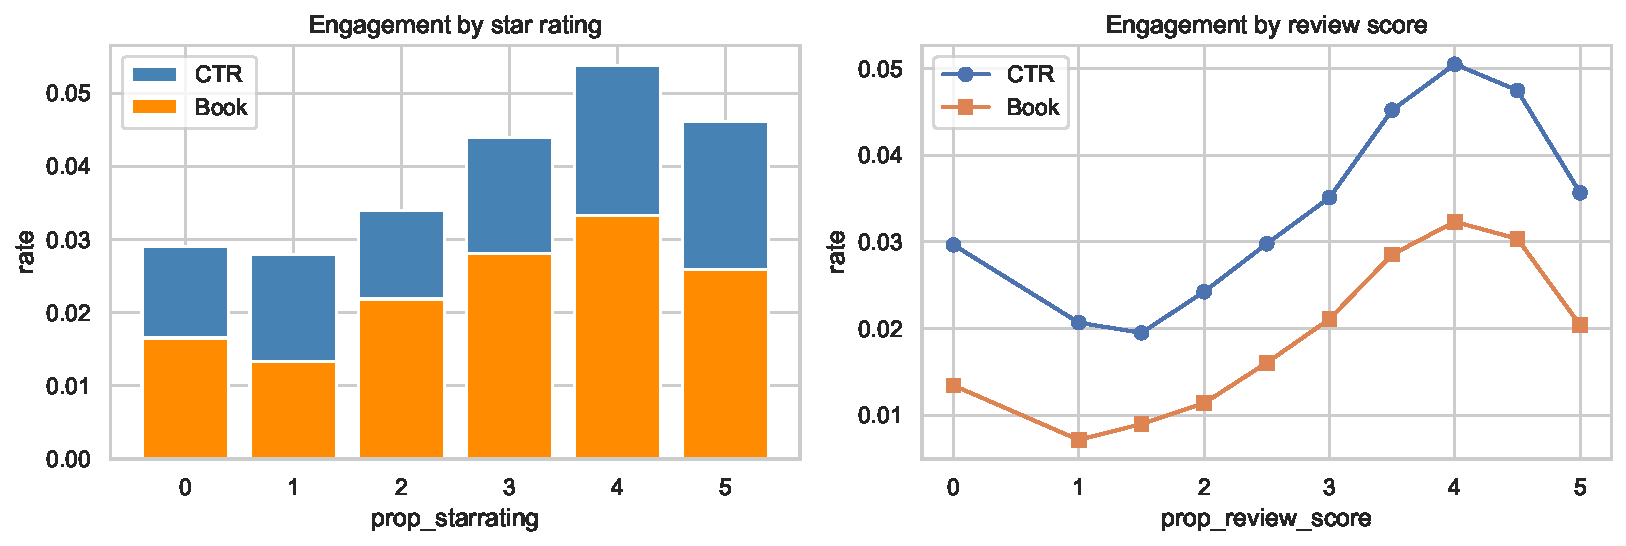
\includegraphics[width=\textwidth]{figures/property_quality.pdf}
\caption{Click-through and booking rate by star rating (left) and review score (right).}
\label{fig:quality}
\end{figure}

\subsection{Missing Values}
Missingness varies a lot across columns (Fig.~\ref{fig:missing}). The competitor columns (\texttt{comp*\_rate}, \texttt{comp*\_inv}, \texttt{comp*\_rate\_percent\_diff}) are missing in 52\% to 98\% of rows, since not every competitor has data for every search. Visitor history (\texttt{visitor\_hist\_starrating}, \texttt{visitor\_hist\_adr\_usd}) is missing 95\% of the time, and \texttt{srch\_query\_affinity\_score} is absent in 94\% of rows. The distance \texttt{orig\_destination\_distance} is missing in 32\% of rows and \texttt{prop\_location\_score2} in 22\%. We will treat missingness as informative (adding indicator flags) and impute the remaining values using the per-country first quartile, as suggested by \cite{DBLP:journals/corr/LiuXZYPLSW13}.

\begin{figure}[ht]
\centering
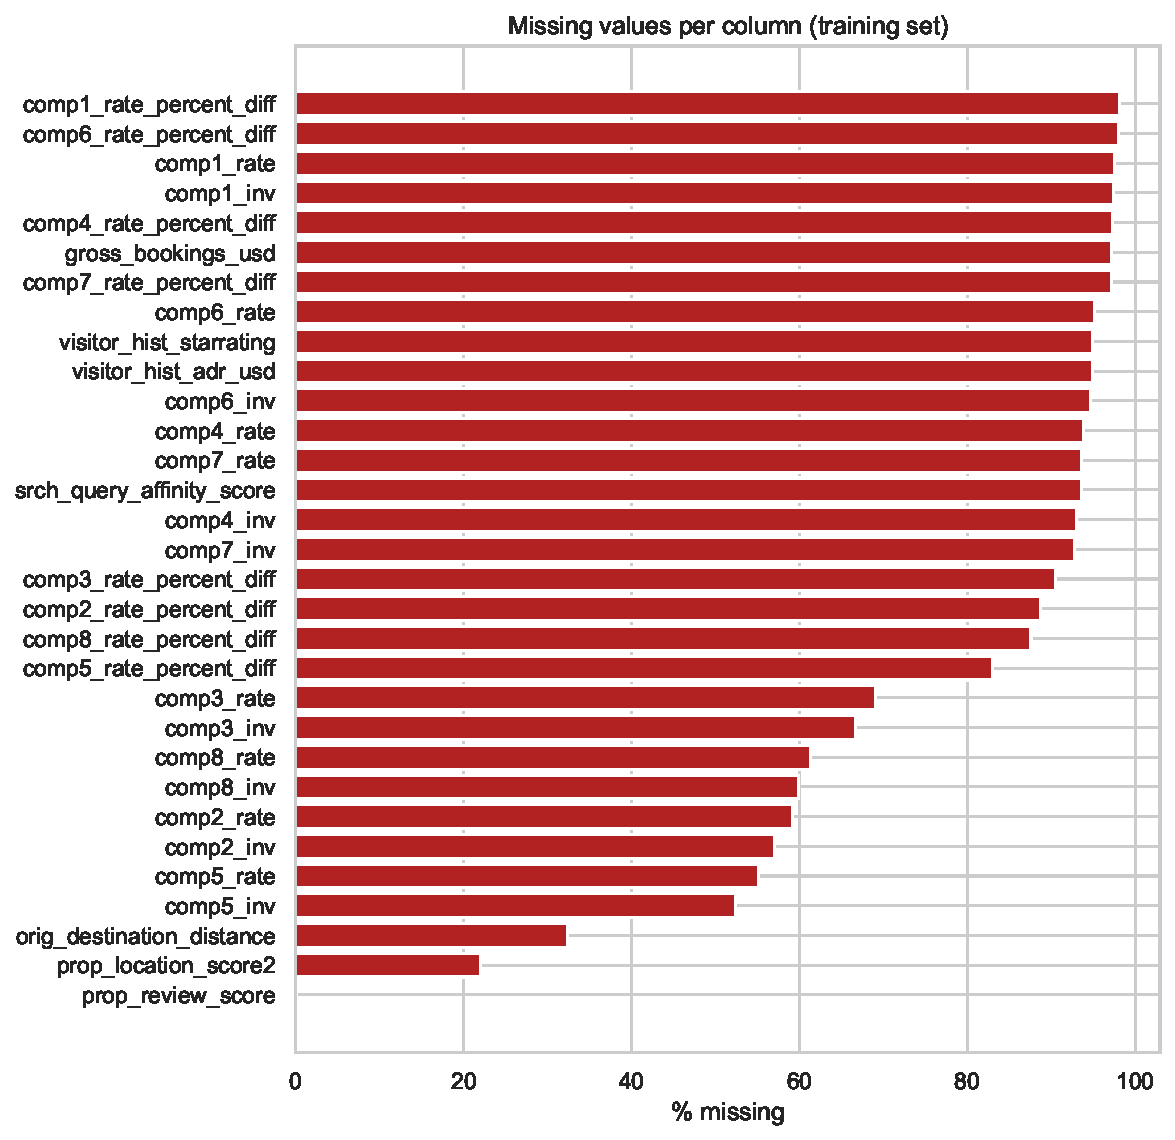
\includegraphics[width=0.85\textwidth]{figures/missingness.pdf}
\caption{Percentage of missing values per column in the training set.}
\label{fig:missing}
\end{figure}




\section{Data Preparation}

\color{blue}You’ll certainly need to work on the dataset, to create, modify or add new features. For instance, you might want to compare the different properties that resulted from the search instead of learning from them one by one. There are certain attributes with a large amount of missing values, do they still provide useful information? And how will you handle a missing 4 value if this shows to be the case? Finally, in order to test your approach (since you do not know the answers for the test set) you will need to split up your data to test your approach yourself before you generate your answers on the test set. Of course, you are also allowed to use external data sources if you find ones that are useful. In case you get inspired by previous work on this competition, please make sure you properly cite the sources you base your approach on.\color{black}

The data preparation step turns the raw training and test sets into two clean tables that share exactly the same set of features. All transformations are applied through a single helper function so that the pipeline can be reproduced on the test set without leakage from the validation data. The final dataset has 82 columns, of which 30 are engineered.

\subsection{Outlier Handling}
The exploratory analysis showed that \texttt{price\_usd} contains values up to about \$1.97\,M and 31 zero-priced rows. Both extremes are clearly encoding errors and would dominate any regression that involves the price. We therefore clip the column to the realistic interval $[1, 5000]$ and store the cleaned values in a new column \texttt{price\_clipped}. We also keep a logarithmic version, \texttt{log\_price} = $\log(1 + \texttt{price\_clipped})$, since the price distribution is heavily skewed and many models work better on a logarithmic scale. We deliberately do not drop the outlying rows because each query needs to keep all of its results to compute relative features such as ranks within the query.

\subsection{Missing Value Handling}
The exploratory analysis revealed that missingness is widespread but not random: it is concentrated in competitor columns, in visitor history and in \texttt{srch\_query\_affinity\_score}. We adopt three different strategies depending on the nature of the column.

\begin{itemize}
    \item \textbf{Indicator flags.} For every column with a non-trivial fraction of missing values we add a binary flag \texttt{<col>\_missing}. This way the model can learn that the very fact of being missing carries information, for example a user without history is rarely a returning customer.
    \item \textbf{Per-country first-quartile imputation.} For numerical attributes such as \texttt{prop\_review\_score}, \texttt{prop\_location\_score2}, \texttt{orig\_destination\_distance}, \texttt{srch\_query\_affinity\_score} and the visitor history columns, we replace the missing values with the first quartile computed inside the same \texttt{prop\_country\_id}. This idea is taken from the reference paper \cite{DBLP:journals/corr/LiuXZYPLSW13} and is more robust than mean imputation because the distributions are skewed and contain outliers. If a country has no observation for a given column we fall back to the global first quartile.
    \item \textbf{Zero imputation for competitor differences.} The columns \texttt{comp1\_rate\_percent\_diff} to \texttt{comp8\_rate\_percent\_diff} are missing whenever the competitor itself is not present, so we fill them with zero, which corresponds to no price difference.
\end{itemize}

The first-quartile lookup is computed on the training set and then applied to both training and test, so the test set never influences the imputation values.

\subsection{Feature Engineering}
The new features are organised in four groups, all motivated by findings from the exploratory analysis or by the reference paper.

\begin{itemize}
    \item \textbf{Per-query relative features.} The ranking task is intrinsically relative: what matters is how a property compares to its peers in the same search. We compute the price rank inside the query (\texttt{price\_rank\_in\_query}) and z-scores within the query for the price and for the three quality scores \texttt{prop\_starrating}, \texttt{prop\_review\_score} and \texttt{prop\_location\_score2}. The exploratory analysis already showed that the relative price is much more informative than the absolute one.
    \item \textbf{Composite features.} We add normalisations of the price by the duration of the stay (\texttt{price\_per\_night}) and by the number of adults (\texttt{price\_per\_person}), the \texttt{count\_window} feature suggested by \cite{DBLP:journals/corr/LiuXZYPLSW13} as the product of room count and booking lead time, the gap between the current price and the user's historical average daily rate (\texttt{price\_diff\_history}), the gap between the property star rating and the user's historical preference (\texttt{star\_diff\_history}), and the difference between the current log price and the historical log price of the property (\texttt{hist\_price\_delta}).
    \item \textbf{Competitor aggregates.} The eight competitor columns are very sparse, so instead of using them individually we summarise them with three counts: \texttt{n\_comp\_expedia\_cheaper}, \texttt{n\_comp\_expedia\_pricier} and \texttt{n\_comp\_available}. The exploratory analysis confirmed that the first one has a clear monotonic effect on the booking rate.
    \item \textbf{Simple flags.} A \texttt{domestic} flag is set when the visitor and the property share the country, and \texttt{has\_history} marks the rows where the user has previous activity on Expedia. Both proved to correlate with the booking rate.
\end{itemize}

\subsection{Relevance Label and Validation Split}
The competition is a learning-to-rank problem evaluated with NDCG@5. Following the standard convention for this dataset we build a graded relevance label that combines the two original targets:
\[
    \texttt{relevance} =
    \begin{cases}
        5 & \text{if the property was booked,} \\
        1 & \text{if the property was clicked but not booked,} \\
        0 & \text{otherwise.}
    \end{cases}
\]
The values 5 and 1 are the same used by the official Kaggle evaluation script and reflect the fact that a booking is much more valuable than a click. Building this label upfront also lets us apply standard learning-to-rank objectives such as LambdaRank later on.

To reproduce the evaluation procedure offline we hold out 10\% of the queries as a validation set, using \texttt{GroupShuffleSplit} on \texttt{srch\_id}. Splitting at query level (and not at row level) is essential: it prevents the same search from being partially seen during training and ensures that NDCG@5 on the validation set is computed exactly as it will be on the test set. The resulting split keeps the click rate (4.5\%) and the booking rate (2.8\%) very close to the full training set, which means the validation sample is representative.

\subsection{Persistence and Test Set Alignment}
Finally, the same pipeline is applied to the test set using the imputation lookup learned on the training data, and the three resulting tables (training, validation and test) are saved as Parquet files inside a \texttt{processed/} folder. Saving in Parquet rather than CSV is a deliberate choice: it keeps column types intact (so the new \texttt{int8} flags do not get cast back to \texttt{float64}) and reduces the disk footprint by about a factor of three, which is convenient since the training table alone has 4.96\,M rows and 82 columns.

\section{Modeling And Evaluation}

\color{blue}Naturally, once you prepare the dataset, you should be able to build models. You have great freedom to select the techniques you feel are most appropriate and should try at least two
different techniques. At least use one technique that has been discussed during the lec-
ture on Recommender Systems or a variant thereof. The choice of that techniques or al-
ternatives you try might be influenced by how we would like to measure your predictions
at the end (described later in this document). To test how your model performs compared
to other groups, you can upload your answers for the test set on the in class Kaggle web-
site: \href{https://www.kaggle.com/competitions/dmt-2026-2nd-assignment}{\url{https://www.kaggle.com/competitions/dmt-2026-2nd-assignment}}, see previous
instructions for signing up using \href{https://www.kaggle.com/t/4ab3a2ed72ba4b559887b634cebdeca6}{\url{https://www.kaggle.com/t/4ab3a2ed72ba4b559887b634cebdeca6}}.
Note that the score on Kaggle is only for part of the test set, the score on the rest of the test set
will only be disclosed on the final lecture and will form part of your final grade.\color{black}

We are a group of three, so we decided to split the modeling work in three: each of us implemented a different model and then we combined the predictions through an ensemble, an idea taken from the reference paper \cite{DBLP:journals/corr/LiuXZYPLSW13}. Working like this gives us three independent points of view on the same problem and an easy way to measure how much they actually agree.

\subsection{Setup and Evaluation Metric}
All three models are trained on the same prepared training set (\texttt{processed/train.parquet}, around 4.46 million rows over 179{,}815 queries) and evaluated on the held-out validation set (495{,}086 rows over 19{,}980 queries). The feature list is built once and reused by every model: we keep the 79 numeric columns of the prepared dataset, dropping the targets (\texttt{click\_bool}, \texttt{booking\_bool}, \texttt{relevance}, \texttt{gross\_bookings\_usd}), the row identifiers (\texttt{srch\_id}, \texttt{prop\_id}, \texttt{date\_time}) and the leakage column \texttt{position}. The metric is NDCG@5, computed per query and averaged: for each search we sort the candidate hotels by predicted score, take the top five, and compute
\[
    \mathrm{NDCG@5} = \frac{1}{Z}\sum_{i=1}^{5}\frac{\mathrm{rel}_i}{\log_2(i+1)},
\]
where $Z$ is the ideal DCG@5 of the same query. We implement the formula in a small helper \texttt{ndcg\_at\_5} that we call after each model to get a directly comparable number.

\subsection{Model 1: Logistic Regression}
The first model is a class-balanced logistic regression on the booking target (\texttt{booking\_bool}). It is the simplest pointwise baseline: it scores each (query, hotel) pair independently, ignoring the fact that the task is a ranking. We standardise the features with \texttt{StandardScaler}, set \texttt{class\_weight='balanced'} to compensate for the 2.8\% positive rate, and use the predicted booking probability as the score. This model is fast (a few minutes), easy to read and gives us a sanity check: any more sophisticated model should beat it on NDCG@5. On the validation set it reaches NDCG@5 = 0.3466.

\subsection{Model 2: LightGBM with LambdaRank}
The second model is a gradient-boosted ensemble of decision trees trained with the LambdaRank objective. Unlike logistic regression, LambdaRank is a listwise method: at each step it looks at the whole list of candidates of a search and rewards the model when it puts a more relevant hotel above a less relevant one. We use the graded \texttt{relevance} label (5 for booked, 1 for clicked, 0 otherwise) and pass the per-query group sizes through the \texttt{group=} argument of \texttt{LGBMRanker}. We train up to 500 trees with \texttt{learning\_rate=0.05} and \texttt{num\_leaves=63}, and rely on early stopping on the validation NDCG@5 (patience 30) so we do not have to tune the number of trees by hand. The reference paper uses LambdaMART with similar hyperparameters and reports it as the best single model, so we expect this to be our strongest base model. On the validation set it reaches NDCG@5 = 0.3935 after 398 trees.

\subsection{Model 3: Matrix Factorization (SVD)}
The third model is a matrix factorization, the technique presented in the Recommender Systems lecture. We build a sparse implicit-feedback matrix $R$ where rows are unique \texttt{srch\_destination\_id} values and columns are unique \texttt{prop\_id} values; each cell counts $2 \cdot \#\text{bookings} + 1 \cdot \#\text{clicks}$ observed in the training data. We then run a truncated SVD with $k=32$ components, which gives us a destination matrix $U \in \mathbb{R}^{n_d \times k}$ and a property matrix $V \in \mathbb{R}^{n_p \times k}$. The score for a candidate hotel is the dot product $U_d \cdot V_p$ of its destination and property latent vectors. The intuition is that destinations that are typically booked together share latent factors with their popular hotels, so the dot product captures a notion of destination-hotel affinity that the per-row models cannot see. Rows of the test set with an unseen \texttt{srch\_destination\_id} or \texttt{prop\_id} get a score of zero. On the validation set the SVD alone reaches NDCG@5 = 0.2719, which is the weakest of the three but, as we will see, it still adds useful diversity to the ensemble.

\subsection{Ensemble}
Each model produces a score on a different scale: a probability in $[0, 1]$ for the logistic regression, an unbounded log-odds for LightGBM, and a small dot product for SVD. To make them comparable we apply a per-query z-score normalization, the same trick used by the reference paper for their winning ensemble. For every search we replace each model's score with $\tilde{s}_m = (s_m - \mu_q) / \sigma_q$, where the mean and standard deviation are computed inside that single search. Then we combine the three normalised scores with a non-negative weighted sum
\[
    s_\text{ensemble} = w_1 \tilde{s}_\text{LR} + w_2 \tilde{s}_\text{LGBM} + w_3 \tilde{s}_\text{SVD},
\]
with $w_1 + w_2 + w_3 = 1$. The weights are tuned by a small grid search (step 0.1) over the validation NDCG@5. The best combination is $w_\text{LGBM} = 0.8$, $w_\text{SVD} = 0.2$, $w_\text{LR} = 0.0$, which gives NDCG@5 = 0.3999. The grid search dropped the logistic regression entirely, but kept a non-trivial weight for the SVD: that is exactly the kind of diversity we hoped to see, the SVD complements the ranker by adding destination-level information.

\subsection{Results}
Table~\ref{tab:results} summarises the validation NDCG@5 of each model and of the ensemble. The ensemble is the best, beating the strongest single model (LightGBM) by about 0.6 NDCG points. Final test predictions are produced by the ensemble and written to \texttt{submission.csv} (4{,}959{,}183 rows, 199{,}549 unique searches), ready to be uploaded to the Kaggle leaderboard.

\begin{table}[ht]
\centering
\renewcommand{\arraystretch}{1.15}
\caption{Validation NDCG@5 for each model and for the ensemble.}\label{tab:results}
\begin{tabular}{|l|c|}
\hline
\textbf{Model} & \textbf{Validation NDCG@5} \\
\hline
Logistic Regression                  & 0.3466 \\
\hline
LightGBM with LambdaRank             & 0.3935 \\
\hline
Matrix Factorization (SVD, $k=32$)   & 0.2719 \\
\hline
Ensemble ($w_\text{LGBM}=0.8$, $w_\text{SVD}=0.2$) & \textbf{0.3999} \\
\hline
\end{tabular}
\end{table}

\section{Deployment}

\color{blue}While we do not go into real deployment, we do want you to:
\begin{itemize}
    \item Apply one of the ethical AI techniques discussed in class to detect and mitigate possible
biases in your model. You may choose any type of bias (e.g., variable performance
across user groups like business travelers vs. families or underrepresentation of certain
hotels). In your report, describe:
\begin{enumerate}
    \item How you detected the bias (include relevant fairness metrics)
    \item Which bias mitigation technique you applied (pre-processing or post-processing)
    \item How effective the mitigation was based on your evaluation results\color{black}
\end{enumerate}
\end{itemize}
\color{black}

\section{What We Learned}

\color{blue}Please describe what skills and knowledge you have gained from this assignment, what were the main difficulties, expected and unexpected outcomes of your
experiments, etc.\color{black}


%
% ---- Bibliography ----
%
% BibTeX users should specify bibliography style 'splncs04'.
% References will then be sorted and formatted in the correct style.
%
\bibliography{references}
\bibliographystyle{splncs04}
% \bibliography{mybibliography}

\end{document}
